
%(BEGIN_QUESTION)
% Copyright 2015, Tony R. Kuphaldt, released under the Creative Commons Attribution License (v 1.0)
% This means you may do almost anything with this work of mine, so long as you give me proper credit

Read and outline the ``DP Transmitter Applications'' subsection of the ``Differential Pressure Transmitters'' section of the ``Continuous Pressure Measurement'' chapter in your {\it Lessons In Industrial Instrumentation} textbook.  Note the page numbers where important illustrations, photographs, equations, tables, and other relevant details are found.  Prepare to thoughtfully discuss with your instructor and classmates the concepts and examples explored in this reading.

\underbar{file i03901}
%(END_QUESTION)





%(BEGIN_ANSWER)


%(END_ANSWER)





%(BEGIN_NOTES)

Pipes or tubes connecting a pressure instrument to a process line are called {\it impulse lines}, {\it gauge lines}, or {\it sensing lines}.

\vskip 10pt

When a DP transmitter is connected across a filter, it is able to detect filter clogging by the pressure difference across the filter, rejecting the filter's common-mode pressure.  The ``H'' port connects to the upstream line, while the ``L'' port connects to the downstream line.

\vskip 10pt

To measure positive gauge pressure, a DP transmitter's ``H'' port is connected to the process vessel while the ``L'' port is vented to atmosphere.  Special ``gauge'' models of pressure transmitter omit a ``L'' port and instead provide a small vent hole for the ``L'' side of the sensing capsule.

\vskip 10pt

To measure absolute pressure, a DP transmitter's ``H'' port is connected to the process while the ``L'' side of the sensing capsule is a sealed vacuum chamber.

\vskip 10pt

To measure negative gauge pressure (vacuum), a DP transmitter's ``L'' port is connected to the process vessel while the ``H'' port is vented to atmosphere.  Note that it is possible to range an electronic pressure transmitter such that a negative pressure is the high-range value, allowing the ``H'' port to be connected to the vacuum vessel.

\vskip 10pt

To infer liquid level, a DP transmitter's ``H'' port is connected to the bottom of a liquid-holding process vessel.  More level (height) equals more hydrostatic pressure by the formula $P = \rho g h$.  The ``L'' port may be connected to the top of the vessel in order to reject any gas pressure within the vessel.

\vskip 10pt

To infer fluid flow, connect a DP transmitter across a restriction such as an orifice.  The more flow, the greater the pressure drop across the restriction.










\vskip 20pt \vbox{\hrule \hbox{\strut \vrule{} {\bf Suggestions for Socratic discussion} \vrule} \hrule}

\begin{itemize}
\item{} {\bf Identify ways in which any of these DP measurement applications (especially any of the inferential measurements) may fail: that is, yield incorrect measurements due to abnormal conditions.}
\item{} Explain how we know which side of a DP transmitter to {\it vent} in certain applications?
\item{} When using a DP transmitter to measure gauge pressure, is it permissible to plug (seal) the ``L'' port of the transmitter, or must that port be vented to atmosphere?  Explain your answer in detail.
\item{} If a {\it gauge pressure} transmitter were tested on a bench (vented) at sea level versus tested on a bench (vented) in Denver, Colorado (altitude = 1 mile), would the transmitter register differently between those two locations? 
\item{} If an {\it absolute pressure} transmitter were tested on a bench (vented) at sea level versus tested on a bench (vented) in Denver, Colorado (altitude = 1 mile), would the transmitter register differently between those two locations? 
\item{} If a DP transmitter were used in an application where the common-mode pressure was 500 PSI but the differential pressure was only about 1 PSI, would a technician calibrating this transmitter on a bench have to apply a full 500 PSI to it?
\item{} If a DP transmitter were used in an application to sense a vacuum, would a technician calibrating this transmitter on a bench have to apply a vacuum to check its calibration, or could the technician use a pressure instead?
\item{} Is it possible to configure a DP transmitter to sense pressure in a process vessel where the expected process fluid pressure range encompasses both positive pressure and negative (vacuum) pressure?  For example, suppose a process vessel normally experienced pressure variations from $-10$ PSI to +10 PSI.  How could you use a DP transmitter to cover that full range of pressure?  A real-world example of this is measuring manifold pressure in a turbocharged gasoline engine, where the range of pressure extends from vacuum (approximately $-10$ PSI) to positive pressure (+15 PSI or more).
\item{} Explain what it means to {\it infer} a measurement rather than directly measure something.
\item{} Is it possible to configure a DP transmitter to measure two-directional flow through an orifice plate?
\end{itemize}




















\vfil \eject

\noindent
{\bf Summary Quiz:}

How much {\it differential pressure} does the DP transmitter measure between the two pressure vessels in this application?

$$\includegraphics[width=15.5cm]{i03901x01.eps}$$

\begin{itemize}
\item{} +75 PSI
\vskip 5pt 
\item{} -14 PSI
\vskip 5pt 
\item{} -61 PSI
\vskip 5pt 
\item{} +61 PSI
\vskip 5pt 
\item{} +14 PSI
\vskip 5pt 
\item{} -75 PSI
\end{itemize}



%INDEX% Reading assignment: Lessons In Industrial Instrumentation, Differential Pressure Transmitters

%(END_NOTES)


